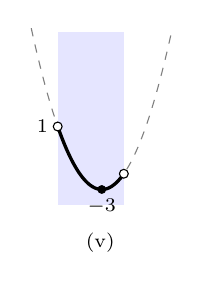
\begin{tikzpicture}[x=2.8mm,y=2mm]
\fill[blue!10] (0,-4) rectangle (3,7);
\ax{-1.6}{5.6}{-4}{7}
\draw[dashed,gray,domain=-1.2:5.2,samples=80] plot (\x,{(\x-2)^2-3});
\draw[very thick,domain=0:3,samples=80] plot (\x,{(\x-2)^2-3});
\fill (2,-3) circle (1.6pt);
\node[below] at (2,-3){\scriptsize $-3$};
\draw[fill=white] (0,1) circle (1.6pt);
\node[left] at (0,1){\scriptsize 1};
\draw[fill=white] (3,-2) circle (1.6pt);
\node[below] at (current bounding box.south){\scriptsize (v)};
\end{tikzpicture}